\documentclass{article}

\usepackage[english]{babel}
\usepackage{amsthm}
\usepackage{amssymb}
\usepackage{graphicx}

\usepackage{enumerate} % to be able to use a parametrised enumerate
                       % environment where we can specify how the
                       % items in the environment are labelled.

\newcommand{\nat}{\mathbb{N}}

\title{Homework 3}
\author{CPSC450, Fall2020}
\date{September 2, 2020\\
Due: Sunday, September 6, 2020}

\begin{document}
\maketitle

\begin{enumerate}

\item Let $G = (V, \Sigma, P, S)$, where $V = \{S, A, B\}$, $\Sigma =
  \{a, b\}$, and $P$ is the set of rules:
\begin{eqnarray*}
S &\rightarrow& ASB \mid \lambda\\
A &\rightarrow& aAb \mid \lambda\\
B &\rightarrow& bBa \mid ba.
\end{eqnarray*}
\begin{enumerate}
\item\label{parta} Give a derivation of $aabbba$.
\newline S $\rightarrow$ ASB
\newline $\rightarrow$ aAbSB $A->aAb$
\newline $\rightarrow$ aaAbbB $A->aAb $ \& $ S-> \lambda$
\newline $\rightarrow$ aabbba $B->ba  $ \& $ A-> \lambda$
\item Build a derivation tree for the derivation in
  part~(\ref{parta}).\newline
  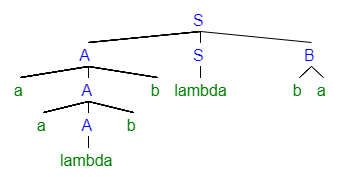
\includegraphics[scale=0.75]{Derivation.png}
\item Use set notation to define $L(G)$.
\newline $L(G) = \{a^nb^nb^ma^m|n\geq0, m>0\}$
\end{enumerate}

(You can create an image file of the derivation using any drawing
software, and then include the image in the \LaTeX\ document for your
solutions. The \LaTeX\ tutorial I created has examples of including
images in \LaTeX\ documents.)
% The use of "\ " after "\LaTeX" is to typeset a blank space after
% typesetting the way LaTeX is written.

\item Let $G = (V, \Sigma, P, S)$, where $V = \{S, B\}$, $\Sigma =
  \{a, b\}$, and $P$ is the set of rules:
\begin{eqnarray*}
S &\rightarrow& aSB \mid aB\\
B &\rightarrow& bb \mid b.
\end{eqnarray*}
Use set notation to define $L(G)$.
\newline $L(G) = \{a^nb^m|n>0,m>0\}$

\item Construct a grammar over $\{a, b, c\}$ whose language is
  $\{a^nb^ic^m \mid (n, m \in \nat) \mbox{ and } (i = m+n)\}$.
  \newline $a^ni^{m+n}c^m$
  \newline S $\rightarrow$ A
  \newline A $\rightarrow$ aAB$|$bAB$|\lambda$
  \newline B $\rightarrow$ c
  
  \item Let $G = (V, \Sigma, P, S)$, where $V = \{S, A\}$, $\Sigma =
  \{a, b, c\}$, and $P$ is the set of rules:
\begin{eqnarray*}
S &\rightarrow& aSbb \mid A\\
A &\rightarrow& cA \mid c.
\end{eqnarray*}
Use set notation to define $L(G)$.
\newline $L(G) = \{a^nb^{2n}c^m|n\geq0,m>0\}$

\item Construct a grammar over $\{a, b, c\}$ whose language is
  $\{a^nb^{2n}c^m \mid n, m \in (\nat \backslash \{0\})\}$.
  \newline Smallest string in the set, abbc. Let G = (V, $\Sigma$,P,S), where V = $\{S,A,B\}$, $\Sigma \{a,b,c\}$, and P is the set of rules:
  \newline L(G) = (V,$\Sigma$,S,P)
  \newline S $\rightarrow$ aAbbcB
  \newline A $\rightarrow$ aAbb$|\lambda$
  \newline B $\rightarrow$ cB$|\lambda$
\item Consider the grammar $G(V, \Sigma, S, P)$ where $V = \{S, A\}$,
  $\Sigma = \{a, b, c, d\}$, and $P$ is given by:
  \begin{eqnarray*}
    S &\rightarrow& aSdd \mid A\\
    A &\rightarrow& bAc \mid bc.
  \end{eqnarray*}

  Prove that the $L(G) = \{a^nb^mc^md^{2n} \mid n \geq 0, m >
     0\}$. 
     \newline S $\rightarrow$ aSdd
     \newline S $\rightarrow$ aAdd
     \newline S $\rightarrow$ abcdd
     \newline\newline S $\rightarrow$ aSdd
     \newline S $\rightarrow$ aaSdddd
     \newline S $\rightarrow$ aaAdddd
     \newline S $\rightarrow$ aabcdddd
     \newline \newline S $\rightarrow$ aSdd
     \newline S $\rightarrow$ aaSdddd
     \newline S $\rightarrow$ aaAdddd
     \newline S $\rightarrow$ aabAcdddd
     \newline S $\rightarrow$ aabbccdddd
     \newline
     \newline 1. A's before b's before c's before d's
     \newline 2. $\geq$ 1 b and c.
     \newline 3. A's before c's and d's
     \newline 4. Number of d's is 2x number of a's
     \newline 5. Number of b's is equal to number of c's
     \newline
     \newline Inductive Hypothesis:
     \newline Induction:
  

\end{enumerate}

\end{document}


